
\section{\trRiemannRoch{}与\trArithmeticGenus}

我们已经见识过\trCechCohomology{}的一些强大用法：证明关于\trGlobalSections{}空间的事情，以及证明\trSerre{}消失。现在我们将会看到，一些经典的构造可以来得又快又便宜。

本节中，我们在一个域 $k$ 上工作。设 $\mathscr{F}$ 是\trProjective{} $k$-\trScheme{} $X$ 上的一个\trCoherentSheaf。回忆记号（\S18.1）$h^i(X,\mathscr{F}):=\dim_k\mathrm{H}^i(X,\mathscr{F})$。由\mbox{定理~18.1.3}，$h^i(X,\mathscr{F})$ 是有限的。（一旦我们经由\trGrothendieck{}凝聚定理~\mbox{18.9.1} 对固有态射得到了这种有限性，本节的论证便可不加改变地推广到\trProper{}的 $X$ 上。）定义 $\mathscr{F}$ 的\textbf{\trEulerCharacteristic}（Euler characteristic）为
\[
\chi(X,\mathscr{F}):=\sum_{i=0}^{\dim X}(-1)^i h^i(X,\mathscr{F}).
\]
在这里与往后我们会反复看到：\trEulerCharacteristic{}比个别的\trCohomology{}群表现得更规矩。一个迹象是：注意，对固定的 $n$ 与 $m\ge 0$，
\[
h^0(\mathbb{P}^n_k,\OO(m))=\binom{n+m}{m}=\frac{(m+1)(m+2)\cdots(m+n)}{n!}.
\]
注意，右边的表达式是变元 $m$ 的一个 $n$ 次多项式。（为备日后参考，也请注意其首项是 $m^n/n!$。）但是，
\[
h^0(\mathbb{P}^n_k,\OO(m))=\frac{(m+1)(m+2)\cdots(m+n)}{n!}
\]
并非对\emph{一切} $m$ 都成立——当 $m\le -n-1$ 时失效。不过你仍可以验证（用\mbox{定理~18.1.2}）：
\[
\chi(\mathbb{P}^n_k,\OO(m))=\frac{(m+1)(m+2)\cdots(m+n)}{n!}.
\]
所以便有这一课：若某个\trCohomology{}群（通常是最高的或最低的那个）在某段范围内表现良好，随后却乱了套，那么多半是因为（i）其实\emph{始终}表现良好的乃是\trEulerCharacteristic，以及（ii）其余的\trCohomology{}群在那段范围内全都消失。

事实上我们将会看到：计算\trCohomology{}群（连 $h^0$ 在内）往往很难，而计算\trEulerCharacteristic{}却可能容易些。因此，把握\trCohomology{}群的一条重要途径便是：先算出\trEulerCharacteristic，再证明\emph{其余}的\trCohomology{}群全都消失。\emph{消失定理}（vanishing theorems）之所以无处不在又举足轻重，道理即在于此。（一条消失定理通常是说：某个\trCohomology{}群在某些条件下消失。）在讨论曲线时，我们就会看到它在起作用。（最早的应用之一将是 \mbox{(19.2.5.1)}。）

下面的练习表明\trEulerCharacteristic{}表现良好的另一种方式：\emph{它在\trExactSequence{}中是\trAdditive{}的}。

\textbf{18.4.A.（练习）}\quad 证明：若 $0\to\mathscr{F}\to\mathscr{G}\to\mathscr{H}\to 0$ 是\trProjective{} $k$-\trScheme{} $X$ 上诸\trCoherentSheaf{}的一个\trExactSequence，则 $\chi(X,\mathscr{G})=\chi(X,\mathscr{F})+\chi(X,\mathscr{H})$。（提示：考虑\trCohomology{}中的\trLongExactSequence。）更一般地，若
\[
0\longrightarrow\mathscr{F}_1\longrightarrow\cdots\longrightarrow\mathscr{F}_n\longrightarrow 0
\]
是诸\trCoherentSheaf{}的一个\trExactSequence，证明
\[
\sum_{i=1}^{n}(-1)^i\chi(X,\mathscr{F}_i)=0.
\]
（这条练习一方面推广了\mbox{练习~1.5.B} 的「正合」情形——考虑 $X=\Spec k$ 的情形——另一方面又在证明中用到它。）

\textbf{18.4.1. 射影曲线上\trLineBundle{}的\trRiemannRoch{}定理。}

\textbf{18.4.B.（重要练习：射影曲线上\trLineBundle{}的\trRiemannRoch{}定理（第一版））}\quad 设 $D=\sum_{p\in C^{\mathrm{reg}}}a_p[p]$ 是域 $k$ 上\trProjective{}（纯维数 $1$）\trCurve{} $C$ 上的一个\trDivisor（其中 $a_p\in\mathbb{Z}$，且除有限多个 $a_p$ 之外均为 $0$）。这里 $C^{\mathrm{reg}}$ 是 $C$ 的维数 $0$ 的\trRegular{}点。定义 $D$ 的\textbf{次数}为
\[
\deg D=\sum a_p\deg p.
\]
（点 $p$ 的次数定义于 \S5.3.8，即剩余域在 $k$ 上的\trFieldExtension{}的次数。）证明
\[
\chi(C,\OO_C(D))=\deg D+\chi(C,\OO_C)
\]
对 $\sum|a_p|$ 归纳（其中 $D=\sum a_p[p]$ 如上）。提示：为证 $\chi(C,\OO_C(D))=\deg p+\chi(C,\OO_C(D-p))$，用 $\OO_C(D)$ 去张量\trClosedSubscheme{}正合列~\mbox{(9.1.2.1)}
\[
0\longrightarrow\OO_C(-p)\longrightarrow\OO_C\longrightarrow\OO_{|p|}\longrightarrow 0
\]
并利用\trEulerCharacteristic{}在\trExactSequence{}中的加性（\mbox{练习~18.4.A}）。

由于\trRegular{}\trCurve{}上每个\trInvertibleSheaf{} $\mathscr{L}$ 都具有 $\OO_C(D)$（对某个 $D$）的形状（见 \S15.4），这条练习威力非常强大。

\textbf{18.4.2.}\ \emph{重要定义：射影曲线上\trLineBundle{}的次数（在 \S18.4.7 中推广）。}\quad 设 $\mathscr{L}$ 是 $k$ 上\trProjective{}\trCurve{} $C$ 上的一个\trInvertibleSheaf（我们对 $C$ 的\trRegularity，乃至\trReducedness，都不作任何假设！）。定义 $\mathscr{L}$ 的\textbf{次数}（记作 $\deg\mathscr{L}$ 或 $\deg_C\mathscr{L}$）为
\[
\deg\mathscr{L}:=\chi(C,\mathscr{L})-\chi(C,\OO_C).
\]
于是我们有了一个次数映射 $\deg\colon\mathrm{Pic}\,C\to\mathbb{Z}$。$C$ 上次数为 $d$ 的\trLineBundle{}全体记作 $\mathrm{Pic}^d\,C:=\deg^{-1}(d)$。

\textbf{18.4.C.（重要而容易的练习：除子的次数＝相应\trLineBundle{}的次数（证成\mbox{注记~16.3.8}））}\quad 设 $\mathscr{L}$ 是 $k$ 上\trProjective{}（纯维数 $1$）\trCurve{} $C$ 上的一个\trInvertibleSheaf，并设 $s$ 是 $\mathscr{L}$ 在 $C$ 上的一个非零\trRational{}\trSection，它在 $C$ 的一切\trSingularPoint{}处都是\trRegular{}的。令 $D$ 为 $s$ 的\trZeros{}与\trPole{}所成的\trDivisor：
\[
D:=\sum_{p\in C}v_p(s)[p].
\]
证明 $\deg\mathscr{L}=\deg D$。特别地，\trRegular{}\trCurve{}上\trLineBundle{}的次数可以这样计算：数一数\emph{任一}不在 $C$ 的某个分量上恒为零的有理截面的零点与极点。

接下来的几条练习给出一些有用的应用。

\textbf{18.4.D.（练习）}\quad 用上面的想法，为\mbox{练习~16.3.E}（射影曲线上的一个非零有理函数拥有同样个数的零点与极点，须以恰当的方式计数）给出一个新的解法。

\textbf{18.4.E.（练习）}\quad 设 $s_1$ 与 $s_2$ 是\trIrreducible\trRegular\trProjective{}\trCurve{} $C$ 上次数为 $d$ 的\trLineBundle{} $\mathscr{L}$ 的两个\trSection，它们没有公共零点。则 $s_1$ 与 $s_2$ 决定一个\trMorphism{} $\pi\colon C\to\mathbb{P}^1_k$。证明：$\pi$ 是\trFinite\trMorphism，且 $\pi$ 的次数为 $d$。（翻译一下：$C$ 上一个二维的、无基点的、次数 $d$ 的\trLinearSystem{}给出 $\mathbb{P}^1$ 的一个次数 $d$ 的\trFinite{}覆盖。）

\textbf{18.4.F.（练习：将在\mbox{练习~18.4.M} 中扩展）}\quad 若 $\mathscr{L}$ 与 $\mathscr{M}$ 是\trRegular\trProjective{}\trCurve{} $C$ 上的两个\trLineBundle，证明 $\deg(\mathscr{L}\otimes\mathscr{M})=\deg\mathscr{L}+\deg\mathscr{M}$。（提示：选取 $\mathscr{L}$ 与 $\mathscr{M}$ 的非零\trRational{}\trSection。）

\textbf{18.4.3.}\ \emph{注记：「次数」映射 $\mathrm{Pic}\to\mathbb{Z}$ 是同态。}\quad 于是，对（域 $k$ 上的）\trRegular\trProjective{}\trCurve{} $C$，次数映射 $\deg\colon\mathrm{Pic}\to\mathbb{Z}$ 是\trAbelianGroups{}的一个\trHomomorphism。（这一结果将在\mbox{练习~18.4.M} 中推广到 $k$ 上的一切\trProper{}\trCurve。）

\textbf{18.4.G.（练习）}\quad 设 $\pi\colon C\to C'$ 是\trIntegral\trProjective\trRegular{}\trCurve{}之间次数为 $d$ 的\trMorphism，而 $\mathscr{L}$ 是 $C'$ 上的一个\trInvertibleSheaf。证明：$\deg_C\pi^*\mathscr{L}=d\deg_{C'}\mathscr{L}$。提示：用 $\mathscr{L}$ 的任一非零\trRational{}\trSection{} $s$ 计算 $\deg_{C'}\mathscr{L}$，并用 $\pi^*\mathscr{L}$ 的\trRational{}\trSection{} $\pi^*s$ 计算 $\deg_C\pi^*\mathscr{L}$。注意：零点拉回为零点，极点拉回为极点。视你的进路而定，\mbox{练习~16.3.D} 或许帮得上忙。

\textbf{18.4.H.}\ \extrahard\ \textbf{（练习：次数的复解析解释；仅供分析背景足够者）}\quad 设 $X$ 是一条\trConnected\trRegular\trProjective{}复曲线。证明：次数映射是下列诸群同态的复合
\[
\begin{tikzcd}[column sep=2.6em]
\mathrm{Pic}\,X \ar[r] & \mathrm{Pic}\,X^{\mathrm{an}} \ar[r, "c_1"] & \mathrm{H}^2(X^{\mathrm{an}},\mathbb{Z}) \ar[r, "{\cap[X^{\mathrm{an}}]}"] & \mathrm{H}_0(X^{\mathrm{an}},\mathbb{Z}) \cong \mathbb{Z}.
\end{tikzcd}
\]
提示：对群 $\mathrm{Pic}\,X$ 的一个\trGenerator{} $\OO(p)$ 证明之，使用显式的\trTransitionFunction。（第一个映射曾在\mbox{练习~14.1.J} 中讨论过。第二个映射把一个\trLineBundle{}送到它的第一\trChern{}类（first Chern class），可以这样来解释：一个\trLineBundle{}的诸\trTransitionFunction{}给出 $\OO^*_{X^{\mathrm{an}}}$ 的一个\trCech{} $1$-\trCycle；这就给出一个映射 $\mathrm{Pic}\,X^{\mathrm{an}}\to\mathrm{H}^1(X^{\mathrm{an}},\OO^*_{X^{\mathrm{an}}})$。再把它与相应于\trExponentialSequence{}~\mbox{(2.4.9.1)} 的\trCohomology{}\trLongExactSequence{}中的映射 $\mathrm{H}^1(X^{\mathrm{an}},\OO^*_{X^{\mathrm{an}}})\to\mathrm{H}^2(X^{\mathrm{an}},\mathbb{Z})$ 组合起来，便得到第一\trChern{}类映射。）

\textbf{18.4.4. \trArithmeticGenus。}

受几何的推动（见下文的\mbox{奇迹~18.4.5}），我们定义维数 $n$ \trScheme{} $X$ 的\textbf{\trArithmeticGenus}（arithmetic genus）为 $p_a(X):=(-1)^n(\chi(X,\OO_X)-1)$。对\trAlgClosedField{}上的\trIntegral\trProjective{}\trCurve，$h^0(X,\OO_X)=1$（\S11.4.7），于是 $p_a(X)=h^1(X,\OO_X)$。（在更高维数，这是一个较不自然的观念。）

我们可以把曲线的\trRiemannRoch{}公式（\mbox{练习~18.4.B}）重述为：
\begin{equation*}\tag{18.4.4.1}\label{eq:riemann-roch-h0-h1}
h^0(C,\mathscr{L})-h^1(C,\mathscr{L})=\deg\mathscr{L}-p_a(C)+1.
\end{equation*}
这是\trRiemannRoch{}公式最常见的一种表述。

\textbf{18.4.5. 奇迹。}\quad 若 $C$ 是一条\trRegular\trIrreducible\trProjective{}复曲线，则相应的复解析对象——一个紧的\trRiemannSurface——有一种叫做\emph{\trGenus} $g$ 的概念，（不严格地说）它就是洞的个数（见图~\ref{fig:genus-3-riemann-surface}）。奇迹般地，在此情形 $g=p_a$（见\mbox{练习~21.4.I}）；因此之故，在讨论\trRegular{}（\trProjective\trIrreducible）曲线时，无论在什么域上，我们都常写 $g$ 来记 $p_a$。我们将在 \S18.6.7 中进一步讨论亏格，届时我们将能在许多有趣的情形计算它。（\trhWarning{}：$\mathbb{P}^1_\mathbb{C}$ 作为 $\mathbb{R}$-\trVariety{}的\trArithmeticGenus{}是 $-1$！）

\begin{figure}[htbp]
\centering
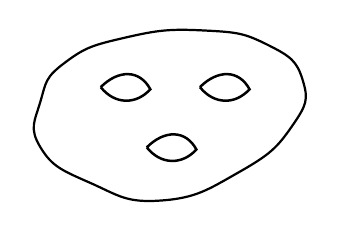
\begin{tikzpicture}[scale=0.9,line width=0.8pt]
  \draw[thick] plot[smooth cycle, tension=0.85] coordinates {
    (-1.7,0.55) (-1.35,1.1) (-0.5,1.45) (0.6,1.55) (1.5,1.35) (2.0,0.85) (1.85,0.2) (1.1,-0.45) (0.0,-0.85) (-1.0,-0.6) (-1.7,-0.1)};
  \draw[line width=0.9pt] (-0.85,0.75) .. controls (-0.6,1.0) and (-0.3,1.0) .. (-0.15,0.72) .. controls (-0.35,0.5) and (-0.65,0.5) .. (-0.85,0.75);
  \draw[line width=0.9pt] (0.55,0.75) .. controls (0.8,1.0) and (1.1,1.0) .. (1.25,0.72) .. controls (1.05,0.5) and (0.75,0.5) .. (0.55,0.75);
  \draw[line width=0.9pt] (-0.2,-0.1) .. controls (0.05,0.15) and (0.35,0.15) .. (0.5,-0.13) .. controls (0.3,-0.35) and (0.0,-0.35) .. (-0.2,-0.1);
\end{tikzpicture}
\caption{一个亏格 $3$ 的\trRiemannSurface{}。（依原书手绘图重绘。）}\label{fig:genus-3-riemann-surface}
\end{figure}

\textbf{18.4.6. \trCoherentSheaf{}的次数（例如\trVectorBundle{}的次数）。}

设 $C$ 是域 $k$ 上的一条\trIrreducible\trReduced{}\trCurve（可能奇异）。若 $\mathscr{F}$ 是 $C$ 上的一个\trCoherentSheaf，回忆一下（\S14.3.3）：$\mathscr{F}$ 的\emph{\trRank}（记作 $\operatorname{rank}\mathscr{F}$）是它在 $C$ 的\trGenericPoint{}处的\trRank。

\textbf{18.4.7.}\ \emph{\trhDefinition{。}}\quad 若 $C$ 是\emph{射影}的，定义 $\mathscr{F}$ 的\textbf{次数}为
\begin{equation*}\tag{18.4.7.1}\label{eq:degree-coherent-sheaf}
\deg\mathscr{F}=\chi(C,\mathscr{F})-(\operatorname{rank}\mathscr{F})\cdot\chi(C,\OO_C).
\end{equation*}
陈述 \eqref{eq:degree-coherent-sheaf} 常被称作射影曲线上\textbf{\trCoherentSheaf{}的\trRiemannRoch{}定理}（或\trVectorBundle{}的\trRiemannRoch{}定理）。

若 $\mathscr{F}$ 是一个\trInvertibleSheaf（或者，更一般地，若\trRank{}在每个\trIrreducibleComponent{}上都相同），我们便可以去掉\trIrreducibility{}假设。

\textbf{18.4.I.（容易的练习）}\quad 证明：次数（作为固定曲线 $C$ 上诸\trCoherentSheaf{}的函数）在\trExactSequence{}中是\trAdditive{}的。

\textbf{18.4.J.（练习）}\quad 若 $\mathscr{F}$ 是 $C$ 上的一个\trTorsion\trSheaf，证明 $\deg\mathscr{F}\ge 0$，且等号成立当且仅当 $\mathscr{F}=0$。

\textbf{18.4.K.（练习）}\quad 若 $k=\overline{k}$，而 $\mathscr{F}$ 是 $C$ 上的一个\trTorsion\trSheaf，证明 $\deg\mathscr{F}=\ell(\mathscr{F})$。（$\mathscr{F}$ 的\trLength{} $\ell(\mathscr{F})$ 定义于 \S6.5.8。）若 $k\ne\overline{k}$，会出什么岔子？

\textbf{18.4.L.}\ \hard\ \textbf{（练习）}\quad 设 $C$ 是域 $k$ 上的一个\trProjective{}\trCurve，$\mathscr{L}$ 是 $C$ 上的一个\trLineBundle，$\mathscr{F}$ 是 $C$ 上的一个\trCoherentSheaf。用下列步骤证明：$\chi(C,\mathscr{L}\otimes\mathscr{F})-\chi(C,\mathscr{F})$ 等于如下乘积对 $C$ 的各\trIrreducibleComponent{} $C_i$ 的求和：$\mathscr{L}$ 在 $C_i^{\mathrm{red}}$ 上的次数（\trReduction{}定义于 \S9.4.10）乘以 $\mathscr{F}$ 在 $C_i$ 的\trGenericPoint{} $\eta_i$ 处的\trLength（即 $\mathscr{F}_{\eta_i}$ 作为 $\OO_{\eta_i}$-\trModule{}的\trLength——\trLength{}定义于\mbox{定义~6.5.2}）。这条练习完全可以有理由称作\textbf{非既约曲线的\trRiemannRoch}。

（a）先化归到 $\mathscr{F}$ \trSchemeTheoretic{}支撑在 $C^{\mathrm{red}}$ 上的情形（有限型拟凝聚层的概形论支撑，你在\mbox{练习~9.1.N} 中定义过），做法是：证明所谓等式的两边在\trShortExactSequence{}中都是\trAdditive{}的，并使用 $\mathscr{F}$ 的如下\trFiltration
\[
0=\mathscr{I}^r\mathscr{F}\subset\mathscr{I}^{r-1}\mathscr{F}\subset\cdots\subset\mathscr{I}\mathscr{F}\subset\mathscr{F}
\]
（其中 $\mathscr{I}$ 是在 $C$ 中切出 $C^{\mathrm{red}}$ 的\trIdealSheaf）。于是我们只须考虑 $C$ 既约的情形。

（b）在这个「既约」情形中，由\mbox{练习~16.2.L}，我们可以写 $\mathscr{L}\cong\OO(\sum_j n_jp_j)$，其中诸 $p_j$ 是与 $\mathscr{F}$ 的\trAssociatedPoint{}互异的\trRegular{}点。用一道恰当的归纳法，证明剩下须证的部分。

\textbf{18.4.M.}\ \hard\ \textbf{（练习）}\quad 若 $\mathscr{L}$ 与 $\mathscr{M}$ 是域 $k$ 上\trProjective{}\trCurve{} $C$ 上的两个\trLineBundle，证明 $\deg_C(\mathscr{L}\otimes\mathscr{M})=\deg_C(\mathscr{L})+\deg_C(\mathscr{M})$。于是次数映射 $\deg\colon\mathrm{Pic}\,C\to\mathbb{Z}$ 是\trAbelianGroups{}的一个\trHomomorphism，这就把\mbox{注记~18.4.3} 加以推广。

\textbf{18.4.8.}\quad 事实上，$k$ 上一切\trProper{}\trCurve{}都是\trProjective{}的（\mbox{注记~19.2.I}），所以在\mbox{练习~18.4.L} 与~\mbox{练习~18.4.M} 中，「射影」可以换成「固有」。正是以这一面目，当我们讨论第 20 章的\trIntersectionTheory{}时，将会用到\mbox{练习~18.4.L}。

\textbf{18.4.9.}\ \emph{曲线上丰富丛的两条性质。}\quad 对于\mbox{练习~18.4.N} 与~\mbox{练习~18.4.O}，要么假设 $C$ 是\trRegular{}的（这样你就可以援引\mbox{注记~18.4.3}），要么使用带星的\mbox{练习~18.4.M}。

\textbf{18.4.N.（练习）}\quad 若 $C$ 是一个\trProjective{}\trCurve，而 $\mathscr{L}$ 是 $C$ 上的一个\trAmple\trLineBundle，证明 $\deg\mathscr{L}>0$。（提示：对 $\mathscr{L}$ \emph{\trVeryAmple}的情形证明之。）

\textbf{18.4.O.（练习）}\quad 设 $\mathscr{L}$ 是\trProper{}\trVariety{} $X$ 上的一个\trBasePointFree\trInvertibleSheaf，从而诱导出某个\trMorphism{} $\phi\colon X\to\mathbb{P}^n$。那么，$\mathscr{L}$ 是\trAmple{}的，当且仅当 $\phi$ 是\trFinite{}的。（提示：若 $\phi$ 是\trFinite{}的，用\mbox{练习~16.2.G}。若 $\phi$ 不是\trFinite{}的，用\mbox{定理~18.1.6} 证明存在一条被 $\phi$ 收缩的曲线 $C$。证明 $\mathscr{L}$ 在 $C$ 上的次数为 $0$。）

\textbf{18.4.10.}\ \hard\ \textbf{扩展例题：万有平面\trConic{}没有有理截面。}\quad 我们用次数的理论来得到一个有趣的推论。我们在一个取定的域 $k$ 上工作。考虑如下的图。
\begin{tikzcd}[row sep=2.8em, column sep=3.2em]
\mathscr{C} \ar[rd] \ar[r, "\mathrm{cl.\,emb.}"] & \mathbb{P}^2\times\mathbb{P}^5 \ar[d] \ar[r] & \mathbb{P}^2 \\
& \mathbb{P}^5 &
\end{tikzcd}
若 $\mathbb{P}^2$ 具有射影坐标 $x_0$、$x_1$、$x_2$，则 $\mathbb{P}^5$ 具有坐标 $a_{00}$、$a_{01}$、$a_{11}$、$a_{02}$、$a_{12}$、$a_{22}$，而 $\mathscr{C}$ 由单独一个方程
\[
a_{00}x_0^2+a_{01}x_0x_1+\cdots+a_{22}x_2^2=0
\]
切出。我们把 $\mathbb{P}^5$ 解释为（$\mathbb{P}^2$ 中的）\trConic{}的参数空间，把 $\mathscr{C}$ 解释为 $\mathbb{P}^5$ 之上的万有\trConic（它把一条\trConic{} $C$ 连同一点 $p\in C$ 一道参数化），并带有\trCanonical{}投射 $\mathscr{C}\to\mathbb{P}^2$。

\textbf{18.4.P.（练习）}\quad 把 $\mathscr{C}$ 解释为 $\mathbb{P}^2$ 上的 $\mathbb{P}^4$-丛（带有两个\trIrreducible\trDivisor，其\trComplement{}是 $\mathbb{A}^2$ 上的 $\mathbb{A}^4$-丛），证明：$\mathscr{C}$ 是一个光滑六维体，且 $\mathrm{Pic}\,\mathscr{C}\cong\mathbb{Z}\times\mathbb{Z}$。

\textbf{18.4.Q.（练习）}\quad 取定一条直线 $\ell\subset\mathbb{P}^2$ 与一个 $k$-值点 $q\in\mathbb{P}^2$。令 $D_\ell$ 为 $\mathscr{C}$ 上相应于 $(C,p)$（其中 $p$ 落在 $\ell$ 上）的\trDivisor。令 $D_q$ 为 $\mathscr{C}$ 上相应于 $(C,p)$（其中 $q\in C$）的\trDivisor。利用你对「$\mathscr{C}$ 是 $\mathbb{P}^2$ 上的 $\mathbb{P}^4$-丛」的描述，证明：$D_\ell$ 与 $D_q$ 生成 $\mathrm{Pic}\,\mathscr{C}$。

\textbf{18.4.R.（练习）}\quad 设 $K$ 是 $\mathscr{C}\to\mathbb{P}^5$ 在点 $r\in\mathbb{P}^5$ 之上的一根\trFiber——也就是说，域 $\kappa(r)$ 上 $\mathbb{P}^2$ 中的一条\trConic。再设 $K$ 是\trIntegral{}的，且 $q$ 与 $\ell$ 都不含于 $K$（这条假设并不必要，但可使问题简化）。证明：$\deg_K\OO(D_q)=0$ 且 $\deg_K\OO(D_\ell)=2$。进而证明：若 $\mathscr{L}$ 是 $\mathscr{C}$ 上的任一\trInvertibleSheaf，则 $\deg_K(\mathscr{L})$ 是偶数。

\textbf{18.4.S.（练习）}\quad 证明：投射 $\pi\colon\mathscr{C}\to\mathbb{P}^5$ 没有有理截面。提示：倘若在 $\mathbb{P}^5$ 的一个\trOpenSubset{} $\mathrm{U}$ 之上存在\trRegular{}\trSection，它将是 $\pi^{-1}(\mathrm{U})$ 上的一个\trDivisor；令 $D$ 为它在 $\mathscr{C}$ 中的\trClosure。证明：$D$ 与 $\pi$ 在 $\mathrm{U}$ 之上的任一\trFiber{}都以重数 $1$ 相交。用\mbox{练习~18.4.R} 导出矛盾。

我们可以按下面这种富于戏剧性的方式重述\mbox{练习~18.4.S}：没有办法写下三个关于 $a_{00},\dots,a_{22}$ 的有理函数 $X_0$、$X_1$、$X_2$，使得
\[
a_{00}X_0^2+a_{01}X_0X_1+\cdots+a_{22}X_2^2=0
\]
除非 $X_0=X_1=X_2=0$。

\trConic{}上有理点的存在问题是一个算术问题。（想想：$x^2+y^2=z^2$。）而我们的解法却是拓扑的。在这个例子中拓扑与算术的统一，是代数几何里一段漫长而富有成果的故事的开端。

\textbf{18.4.11.}\ \hard\ \textbf{\trNumericallyEquivalent、N\'eron--Severi 群、\trNef\trLineBundle、\trNef{}锥与丰富锥。}\quad 设 $X$ 是一个\trProper{} $k$-\trVariety，而 $\mathscr{L}$ 是 $X$ 上的一个\trInvertibleSheaf。若 $i\colon C\hookrightarrow X$ 是 $X$ 的一个一维\trClosed\trReduced{}\trSubscheme，则定义 $\mathscr{L}$ 在 $C$ 上的次数为 $\deg_C\mathscr{L}:=\deg_C i^*\mathscr{L}$。若对一切 $C$ 都有 $\deg_C\mathscr{L}=0$，我们便说 $\mathscr{L}$ 是\textbf{\trNumericallyTrivial}（numerically trivial）的。

\textbf{18.4.T.（练习）}\quad
（a）证明：$\mathscr{L}$ 是\trNumericallyTrivial{}的，当且仅当对 $X$ 中一切\emph{\trIntegral}曲线 $C$ 都有 $\deg_C\mathscr{L}=0$。

（b）证明：若 $\pi\colon X\to Y$ 是一个\trProper\trMorphism，而 $\mathscr{L}$ 是 $Y$ 上的一个\trNumericallyTrivial\trInvertibleSheaf，则 $\pi^*\mathscr{L}$ 在 $X$ 上\trNumericallyTrivial。

（c）证明：$\mathscr{L}$ 是\trNumericallyTrivial{}的，当且仅当 $\mathscr{L}$ 在 $X$ 的每个\trIrreducibleComponent{}上都\trNumericallyTrivial。

（d）证明：若 $\mathscr{L}$ 与 $\mathscr{L}'$ \trNumericallyTrivial，则 $\mathscr{L}\otimes\mathscr{L}'$ 与 $\mathscr{L}^\vee$ 都\trNumericallyTrivial。

\textbf{18.4.12.}\ \emph{\trNumericallyEquivalent。}\quad 由（d）部分，\trNumericallyTrivial\trInvertibleSheaf{}全体构成 $\mathrm{Pic}\,X$ 的一个子群，记作 $\mathrm{Pic}^\tau X$。模去\trNumericallyTrivial\trLineBundle{}所组成的子群而等价的两个线丛，称为\textbf{\trNumericallyEquivalent}（numerically equivalent）的。\footnote{原书此处作「Two lines bundles」，当为「Two line bundles」之误，径改。——译者注}在\trNumericallyEquivalent{}之下稳定的\trInvertibleSheaf{}性质，称为一个\emph{数值性质}（numerical property）。我们将会看到，「\trNef{}性」（nefness）与\trAmpleness{}都是数值性质（分别见\mbox{定义~18.4.13}与\mbox{注记~20.4.2}）。

日后将定义 $X$ 的\emph{N\'eron--Severi 群} $\mathrm{NS}(X)$ 为 $\mathrm{Pic}\,X$ 模代数等价（\mbox{练习~24.7.5}）。（待我们讨论过\trFlatness，便会定义代数等价。）极不平凡的 \textbf{N\'eron--Severi 定理}（或称\textbf{基定理}）断言：$\mathrm{NS}(X)$ 是一个\trFinitelyGenerated{}群。（透彻的现代论述见 [ChJLO]；$\mathbb{C}$ 上的一个较简单的证明见 [GH1, p.~462]。）群 $\mathrm{Pic}\,X/\mathrm{Pic}^\tau X$ 记作 $\mathrm{N}^1(X)$。我们将会看到（\S24.7.5）：它是 $\mathrm{NS}(X)$ 的一个\trQuotient，因而也是有限生成的。由于群 $\mathrm{N}^1(X)$ 显然是阿贝尔群且\trTorsionFree，它是有限秩的自由 $\mathbb{Z}$-\trModule（由主理想整环上有限生成模的分类；见 \S0.3）。$\mathrm{N}^1(X)$ 的\trRank{}称作\textbf{\trPicard{}数}（Picard number），记作 $\rho(X)$（尽管除了在 \S20.2.11 讨论霍奇指标定理时会用到它之外，我们并不需要这个概念）。例如，$\rho(\mathbb{P}^n)=1$，$\rho((\mathbb{P}^1)^n)=n$。我们定义 $\mathrm{N}^1_{\mathbb{Q}}(X):=\mathrm{N}^1(X)\otimes_{\mathbb{Z}}\mathbb{Q}$（于是 $\rho(X)=\dim_{\mathbb{Q}}\mathrm{N}^1_{\mathbb{Q}}(X)$），并把这个群的元素称作\textbf{$\mathbb{Q}$-线丛}（$\mathbb{Q}$-line bundle）——因为文献中缺乏通用的名称。

\textbf{18.4.U.}\ \extrahard\ \textbf{（练习：复情形\trPicard{}数的有限性；仅供背景足够者）}\quad 证明（不用 N\'eron--Severi 定理）：若 $X$ 是一个复的\trProper{}\trVariety，则 $\rho(X)$ 有限，办法是把 $\rho(X)$ 解释为 $\mathrm{H}^2(X,\mathbb{Z})$ 的一个\trSubquotient。提示：证明 $(\mathscr{L},C)$ 在映射 $\mathrm{H}^2(X,\mathbb{Z})\times\mathrm{H}_2(X,\mathbb{Z})\to\mathrm{H}_0(X,\mathbb{Z})\to\mathbb{Z}$ 之下的像是 $\deg_C\mathscr{L}$。提示：想明白如何化归到 $C$ 为光滑射影曲线的情形，然后用\mbox{练习~18.4.H}。

\textbf{18.4.13.}\ \emph{\trhDefinition。}\quad 我们说一个\trInvertibleSheaf{} $\mathscr{L}$ 是\textbf{\trNef}（numerically effective）的，或称 \textbf{nef}，若对一切这样的 $C$ 都有 $\deg_C\mathscr{L}\ge 0$。显然，\trNef{}性（nefness）是一个数值性质。

\textbf{18.4.V.（容易的练习：参看\mbox{练习~18.4.T}）}\quad
（a）证明：$\mathscr{L}$ 是\trNef{}的，当且仅当对 $X$ 中一切\emph{\trIntegral}曲线 $C$ 都有 $\deg_C\mathscr{L}\ge 0$。

（b）证明：若 $\pi\colon X\to Y$ 是一个\trProper\trMorphism，而 $\mathscr{L}$ 是 $Y$ 上的一个\trNef\trInvertibleSheaf，则 $\pi^*\mathscr{L}$ 在 $X$ 上\trNef。（提示：需要用到\mbox{练习~18.4.G}。）

（c）证明：$\mathscr{L}$ 是\trNef{}的，当且仅当 $\mathscr{L}$ 在 $X$ 的每个\trIrreducibleComponent{}上都\trNef。

（d）证明：若 $\mathscr{L}$ 与 $\mathscr{L}'$ \trNef，则 $\mathscr{L}\otimes\mathscr{L}'$ \trNef。于是 $\mathrm{Pic}\,X$ 的\trNef{}元素构成一个\trAbelianSemigroup。

（e）证明：丰富的\trInvertibleSheaf{}都\trNef。

（f）设 $n\in\mathbb{Z}^{>0}$。证明：$\mathscr{L}$ 是\trNef{}的，当且仅当 $\mathscr{L}^{\otimes n}$ \trNef。

\textbf{18.4.W.（练习）}\quad 请定义「$\mathbb{Q}$-线丛是\trNef{}的」的含义。证明：\trNef{} $\mathbb{Q}$-线丛构成 $\mathrm{N}^1_{\mathbb{Q}}(X)$ 中的一个闭锥。它称为\textbf{\trNef{}锥}（nef cone）。

\textbf{18.4.X.（练习）}\quad 描述 $\mathbb{P}^2_k$ 与 $\mathbb{P}^1_k\times_k\mathbb{P}^1_k$ 的\trNef{}锥。（注意，在后一情形中，锥的两条边界对应于收缩一根 $\mathbb{P}^1$ 的\trLinearSystem。这在一般情形下也是真的：不严格地说，与锥的边界相对应的\trLinearSystem{}给出有趣的收缩。另一个例子见\mbox{练习~20.2.F}。）

一个令人惊讶的事实是：$X$ 上的\trInvertibleSheaf{} $\mathscr{L}$ 是否丰富，只依赖于它在 $\mathrm{N}^1_{\mathbb{Q}}(X)$ 中的类，也就是说，只依赖于它与 $X$ 中诸曲线的相交方式。有鉴于此（由于对任意 $n\in\mathbb{Z}^{>0}$，$\mathscr{L}$ 丰富当且仅当 $\mathscr{L}^{\otimes n}$ 丰富；见\mbox{定理~16.2.2}），定义 $\mathbb{Q}$-线丛何时丰富便有其意义。于是由\mbox{练习~16.2.H}，\trAmple{}\trDivisor{}构成 $\mathrm{N}^1_{\mathbb{Q}}(X)$ 中的一个锥，并且由\mbox{练习~18.4.V(e)}，它必然含于\trNef{}锥之中。而事实证明：若 $X$ 是\trProjective{}的，则\trAmple{}\trDivisor{}恰好就是\trNef{}锥的内部。本段中的新事实，是\trKleiman{}丰富性判别法（\mbox{定理~20.4.6}）的推论。
